\documentclass[11pt]{article}
\usepackage{amsmath, amssymb, amsthm}
\usepackage{geometry}
\usepackage{graphicx}
\geometry{margin=1in}
\title{Foundations of Machine Learning -- Lecture 6 Notes}
\author{}
\date{}

\begin{document}
\maketitle

\section*{Support Vector Machines}
Support Vector Machines are a supervised learning method used for classification and regression. 
At their core, SVMs try to separate data into classes with the best possible boundary. 
Imagine you have two groups of points (red and blue) plotted on a graph. 
You want to separate them with a line (in 2D), a plane (in 3D), or more generally, a hyperplane in higher dimensions. 
Many hyperplanes might separate the two groups, but SVM chooses the one with the largest margin — the maximum distance between the hyperplane and the closest points from each class. 
Those closest points are called \textit{support vectors}.

\medskip

Let’s say our model is the following:
\[
f(x) = \text{sign}(w^T x + b)
\]

The hyperplane is defined as:
\[
w^T x + b = 0
\]

For a point $x$:
\[
f(x) = \text{sign}(w^T x + b)
\]

If $f(x) = +1$, the point belongs to one class.  
If $f(x) = -1$, it belongs to the other.

\begin{figure}[h!]
\centering
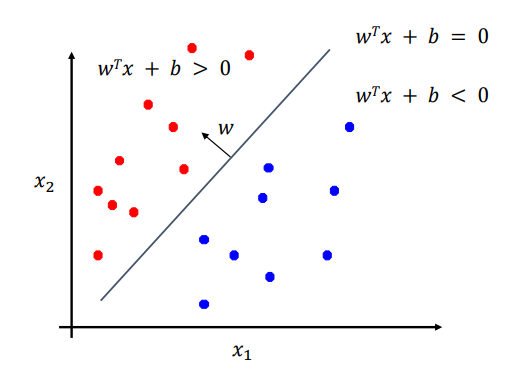
\includegraphics[width=0.6\textwidth]{C:/repos/tex-notes/cs4262/imgs/svm.png}
\caption{Support Vector Machine separating two classes with a hyperplane.}
\end{figure}

\pagebreak
The distance from point $x^(i)$ to our hyperplane seperator is:
\[
r(x^{(i)}) = \frac{1}{\left\lVert w \right\rVert} \, \left| w^T x^{(i)} + b \right|
\]

Margin $\rho$ is the distance between support vectors. And the purpose of SVM is to maximize this.

\[
\rho = \frac{2}{\|w\|}
\]

We also must look at our constraints, we want to maximize this $\rho$, while also making sure all points with $y=-1$ fall below the hyperplane and all points $y=1$ fall above. We write this as:

\[
\begin{cases}
w^T x + b \;\leq\; -\tfrac{\rho}{2}\|w\|, & \text{if } y = -1 \\[6pt]
w^T x + b \;\geq\; \tfrac{\rho}{2}\|w\|, & \text{if } y = 1
\end{cases}
\]

\paragraph{Goal}
\begin{itemize}
    \item Find $w$ and $b$ such that
    \[
    \rho = \frac{2}{\|w\|} \quad \text{is maximized}
    \]
    \item And for all $(x^{(i)}, y^{(i)})$:
    \[
    y^{(i)} \big(w^T x^{(i)} + b\big) \;\geq\; 1 \quad \text{(Equivilent to above piecewise function)}
    \]
\end{itemize}

And now in formulation
\[
 \min_{w,b} \; w^Tw \; \; \text{s.t.} \; \; y^{(i)} \big(w^T x^{(i)} + b\big) \;\geq\; 1, 
\; \; \forall i
\]

\subsection*{What if data is not linearly separable?}

\begin{itemize}
    \item Hard-margin SVM can lead to some issues, for instance the real data may not be perfectly separable (noise, overlap).
    \item So we can allow some ``errors'' in classification and choosing our hyperplane.
\end{itemize}

\paragraph*{Naive Formulation}
\[
\min_{w,b} \; w^T w + C \cdot \#\text{mistakes}
\]
\[
\text{s.t.} \quad y^{(i)}(w^T x^{(i)} + b) \;\geq\; 1, \quad \forall i \setminus \{\text{mistakes}\}
\]

\begin{itemize}
    \item $C$ = trade-off parameter.
        \begin{itemize}
            \item Large $C$: fewer mistakes allowed, narrower margin.
            \item Small $C$: margin prioritized, more mistakes tolerated.
        \end{itemize}
\end{itemize}

\paragraph*{Problems}
\begin{itemize}
    \item Not quadratic programming (QP), since $\#\text{mistakes}$ is discrete.
    \item Uses 0/1 loss:
    \begin{itemize}
        \item Treats all mistakes equally.
        \item No difference between a ``near miss'' and a ``bad mistake.''
    \end{itemize}
\end{itemize}

\paragraph*{Soft-margin SVM}

\begin{itemize}
    \item Introduce slack variables $\xi_i \geq 0$.
        \begin{itemize}
            \item $\xi^{(i)} = 0$: correctly classified and outside the margin.
            \item $0 < \xi^{(i)} \leq 1$: inside the margin but correctly classified.
            \item $\xi^{(i)} > 1$: misclassified point.
        \end{itemize}
    \item $C$: \textbf{trade-off parameter}.
        \begin{itemize}
            \item Large $C$: penalizes violations heavily $\Rightarrow$ fewer mistakes, narrower margin.
            \item Small $C$: allows more violations $\Rightarrow$ wider margin, more tolerance.
        \end{itemize}
\end{itemize}


\[
 \min_{w,b,\{\xi_i\}} \quad w^T w + C \sum_i \xi^{(i)} \; \; \text{s.t} \quad y^{(i)} \big(w^T x^{(i)} + b\big) \;\geq\; 1 - \xi^{(i)}, \; \; \forall i \;\; \xi^{(i)} \;\geq\; 0, \quad \forall i
\]

\begin{itemize}
    \item This formulation is QP!
    \item Distinguishes between a ``near miss'' (small $\xi$) and a ``bad mistake'' (large $\xi$).
\end{itemize}

\[
(w^T x^{(i)} + b) y^{(i)} \;\geq\; 1 - \xi^{(i)}, \quad \forall i
\]
\[
\xi^{(i)} \;\geq\; 0, \quad \forall i
\]

The penalty for misclassification is $C \, \xi^{(i)}$

\begin{figure}[h!]
\centering
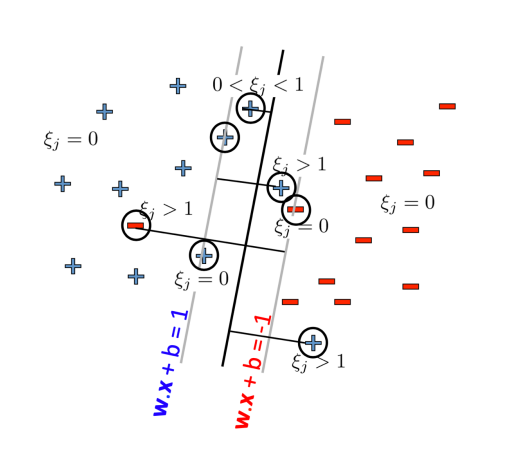
\includegraphics[width=0.4\textwidth]{C:/repos/tex-notes/cs4262/imgs/svm2.png}
\caption{Support Vector Machine separating two classes with a hyperplane.}
\end{figure}

\paragraph*{Hinge Loss}
\[
\xi^{(i)} =
\begin{cases}
1 - \big(w^T x^{(i)} + b\big)y^{(i)}, & \text{not correct} \\[6pt]
0, & \text{correct}
\end{cases}
\]

\[
\Longrightarrow \quad \xi^{(i)} = \max \big(0, \, 1 - (w^T x^{(i)} + b)y^{(i)}\big)
\]

\paragraph*{Optimization Problem}
\[
 \min_{w,b,\{\xi_i\}} \quad w^T w + C \sum_i \xi^{(i)} 
 \;\; \text{s.t.} \;\; y^{(i)} \big(w^T x^{(i)} + b\big) \;\geq\; 1 - \xi^{(i)}, \;\; \forall i, 
 \;\; \xi^{(i)} \;\geq\; 0, \quad \forall i
\]

\section*{Constrained Optimization}

We consider the constrained optimization problem:
\[
\min_{x} f(x) \quad \text{s.t.} \quad g(x) \leq 0, \quad h(x) = 0
\]

This optimization problem is convex if and only if:
\begin{itemize}
    \item $f(x)$ and $g(x)$ are convex,
    \item $h(x)$ is affine, i.e. \(h(x) = w^T x + w_0\)
\end{itemize}
The Lagrangian (dual function) is given by:
\[
\mathcal{L}(x, \alpha, \beta) = f(x) + \alpha g(x) + \beta h(x)
\]
where
\[
\alpha \geq 0, \quad \beta \in \mathbb{R}
\]
are the Lagrange multipliers.\\ 
The Lemma is given by:
\[
\max_{\alpha \geq 0, \beta} \; \mathcal{L}(x, \alpha, \beta) =
\begin{cases}
f(x), & \text{if $x$ is feasible} \\
\infty, & \text{otherwise}
\end{cases}
\]



\subsection*{Strong Duality and KKT Conditions}

If the problem is convex, then any (primal/dual) points that satisfy the
Karush-Kuhn-Tucker (KKT) conditions are primal/dual optimal pairs. The KKT conditions are:

\begin{enumerate}
    \item Stationarity: 
    \[
    \nabla_x \mathcal{L}(x^*, \alpha^*, \beta^*) = 0
    \]
    \item Feasibility:
    \[
    \alpha^* \geq 0, \quad g(x^*) \leq 0, \quad h(x^*) = 0
    \]
    \item Complementary slackness:
    \[
    \alpha^* g(x^*) = 0
    \]
\end{enumerate}

When these conditions hold:
\[
d^* = \max_{\alpha \geq 0, \beta} \min_x \mathcal{L}(x, \alpha, \beta) 
= \min_x \max_{\alpha \geq 0, \beta} \mathcal{L}(x, \alpha, \beta) = p^*
\]

This is called \textbf{strong duality}.


\subsection*{Example: Checking KKT Conditions}

Consider the problem:
\[
\min_x \; x^2 \quad \text{s.t. } x \geq 1
\]

The Lagrangian is:
\[
\mathcal{L}(x, \alpha) = x^2 + \alpha (1 - x)
\]

Suppose $x^* = 1$, $\alpha^* = 2$. Let’s check KKT:

\begin{itemize}
    \item Stationarity: 
    \[
    \nabla_x \mathcal{L}(x, \alpha) = 2x - \alpha = 0 
    \quad \Rightarrow \quad \alpha^* = 2x^* = 2
    \]
    \item Feasibility: 
    \[
    x^* = 1 \geq 1, \quad \alpha^* = 2 \geq 0
    \]
    \item Complementary slackness: 
    \[
    \alpha^* (1 - x^*) = 2(1 - 1) = 0
    \]
\end{itemize}

All KKT conditions are satisfied $\Rightarrow$ $(x^*, \alpha^*) = (1,2)$ is optimal.

\subsection	*{Summary}

For a general constrained optimization problem
\[
\min_{x} f(x) \quad \text{s.t. } g(x) \leq 0, \quad h(x) = 0
\]

\begin{itemize}
    \item \textbf{Non-convex problems:}
    \[
    d^* \leq p^* \quad \text{(Weak Duality)}
    \]
    KKT conditions are necessary but not sufficient.

    \item \textbf{Convex problems:}
    \[
    d^* = p^* \quad \text{(Strong Duality)}
    \]
    KKT conditions are necessary and sufficient.
\end{itemize}

\section*{Applying to SVM}

\textbf{Primal Problem}
\[
\min_{w,b} \;\; \tfrac{1}{2} w^T w 
\quad \text{s.t.} \quad 
y^{(i)} \big(w^T x^{(i)} + b \big) \geq 1
\]
\textbf{Dual Problem}
\[
\max_{\{\alpha^{(i)} \geq 0\}_i} 
\;\; \min_{w,b} \left( 
\tfrac{1}{2} w^T w \;+\; 
\sum_i \alpha^{(i)} \Big[1 - y^{(i)} (w^T x^{(i)} + b) \Big] 
\right)
\]

\subsection*{Solving Dual SVM}

\begin{itemize}
    \item Gradient with respect to $w$:
    \[
    \nabla_w \mathcal{L} = w - \sum_i \alpha^{(i)} x^{(i)} y^{(i)} = 0
    \]
    which gives
    \[
    w^* = \sum_i \alpha^{(i)} y^{(i)} x^{(i)}
    \]

    \item Gradient with respect to $b$:
    \[
    \frac{\partial \mathcal{L}}{\partial b} 
    = - \sum_i \alpha^{(i)} y^{(i)} = 0
    \]
    so
    \[
    \sum_i \alpha^{(i)} y^{(i)} = 0
    \]
\end{itemize}

Substitute $w^*$ into $\mathcal{L}$:

\[
(w^*)^T w^* = 
\left( \sum_i \alpha^{(i)} y^{(i)} x^{(i)} \right)^T
\left( \sum_j \alpha^{(j)} y^{(j)} x^{(j)} \right)
= \sum_{i,j} \alpha^{(i)} \alpha^{(j)} y^{(i)} y^{(j)} \langle x^{(i)}, x^{(j)} \rangle
\]

Hence the dual problem becomes:
\[
\max_{\alpha \geq 0} 
\;\; \sum_i \alpha^{(i)} 
- \tfrac{1}{2} \sum_{i,j} \alpha^{(i)} \alpha^{(j)} y^{(i)} y^{(j)} \langle x^{(i)}, x^{(j)} \rangle
\]

subject to the constraint:
\[
\sum_i \alpha^{(i)} y^{(i)} = 0
\]

Making our dual formulation:
\[
\begin{aligned}
\max_{\alpha} \quad & 
\sum_i \alpha^{(i)} 
- \tfrac{1}{2} \sum_{i,j} \alpha^{(i)} \alpha^{(j)} y^{(i)} y^{(j)} \langle x^{(i)}, x^{(j)} \rangle \\
\text{s.t.} \quad & \alpha^{(i)} \geq 0 \;\; \forall i, \\
& \sum_i \alpha^{(i)} y^{(i)} = 0
\end{aligned}
\]


Only points with $\alpha^{(i)} > 0$ affect $w^*$ (the \textbf{support vectors}).


\subsection*{Getting our solution $w^*$ and $b^*$}

After solving the dual objective and obtaining the optimal multipliers $\alpha$, we can express the optimal $w$ as:
\[
w^* = \sum_i \alpha^{(i)} x^{(i)} y^{(i)}
\]

\subsection*{Recovering $b^*$}
From KKT’s complementary slackness condition:
\[
\alpha^{(i)} g(x^{(i)}) = 0
\quad \Rightarrow \quad
\alpha^{(i)} \Big( y^{(i)} (w^{*T} x^{(i)} + b) - 1 \Big) = 0
\]

- For support vectors ($\alpha^{(i)} > 0$), this gives:
\[
y^{(i)} (w^{*T} x^{(i)} + b^*) = 1
\]

Rearranging, we obtain:
\[
b^{(i)} = y^{(i)} - w^{*T} x^{(i)}
\]

The final bias is computed as an average across support vectors:
\[
b^* = \text{avg}_{\{i : \alpha^{(i)} > 0\}} \; b^{(i)}
\]

\section*{Primal Classifier vs. Dual Classifier}

\subsection*{Primal Classifier}
In primal form, the decision function is:
\[
f(x) = \text{sign}(w^T x + b)
\]

\subsection*{Dual Classifier}
Substituting $w^* = \sum_i \alpha^{(i)} y^{(i)} x^{(i)}$, we obtain the dual classifier:
\[
f(x) = \text{sign}\!\left( \sum_i \alpha^{(i)} y^{(i)} \langle x^{(i)}, x \rangle + b \right)
\]

\subsection*{Key Observations}
\begin{itemize}
    \item Only support vectors ($\alpha^{(i)} > 0$) contribute to the classifier.
    \item The margin is $\tfrac{2}{\|w\|}$, determined entirely by support vectors.
    \item This dual form makes it easy to extend SVMs using kernels by replacing inner products $\langle x^{(i)}, x \rangle$ with kernel functions $K(x^{(i)}, x)$.
\end{itemize}

\textbf{When to use:}
\begin{itemize}
    \item Primal: $n \gg d$ (many samples, few features).
    \item Dual: $d \gg n$ or when using kernels.
\end{itemize}

\end{document}

